\documentclass[12pt,a4paper,twoside]{article}
\usepackage[colorlinks=true]{hyperref}
\usepackage[utf8]{inputenc}
\usepackage[czech]{babel}
\usepackage{pdfpages}
\usepackage{graphicx}
\textwidth 16cm \textheight 25cm
\topmargin -1.3cm 
\oddsidemargin 0cm
\pagestyle{empty}
\begin{document}
\title{Modul převodníku TTLRS48501A}
\author{Jakub Kákona, kaklik@mlab.cz}
\maketitle

\thispagestyle{empty}
\begin{abstract}
Modul je určen pro připojení procesorových modulů na sběrnici RS485.
\end{abstract}

\begin{figure} [htbp]
\begin{center}
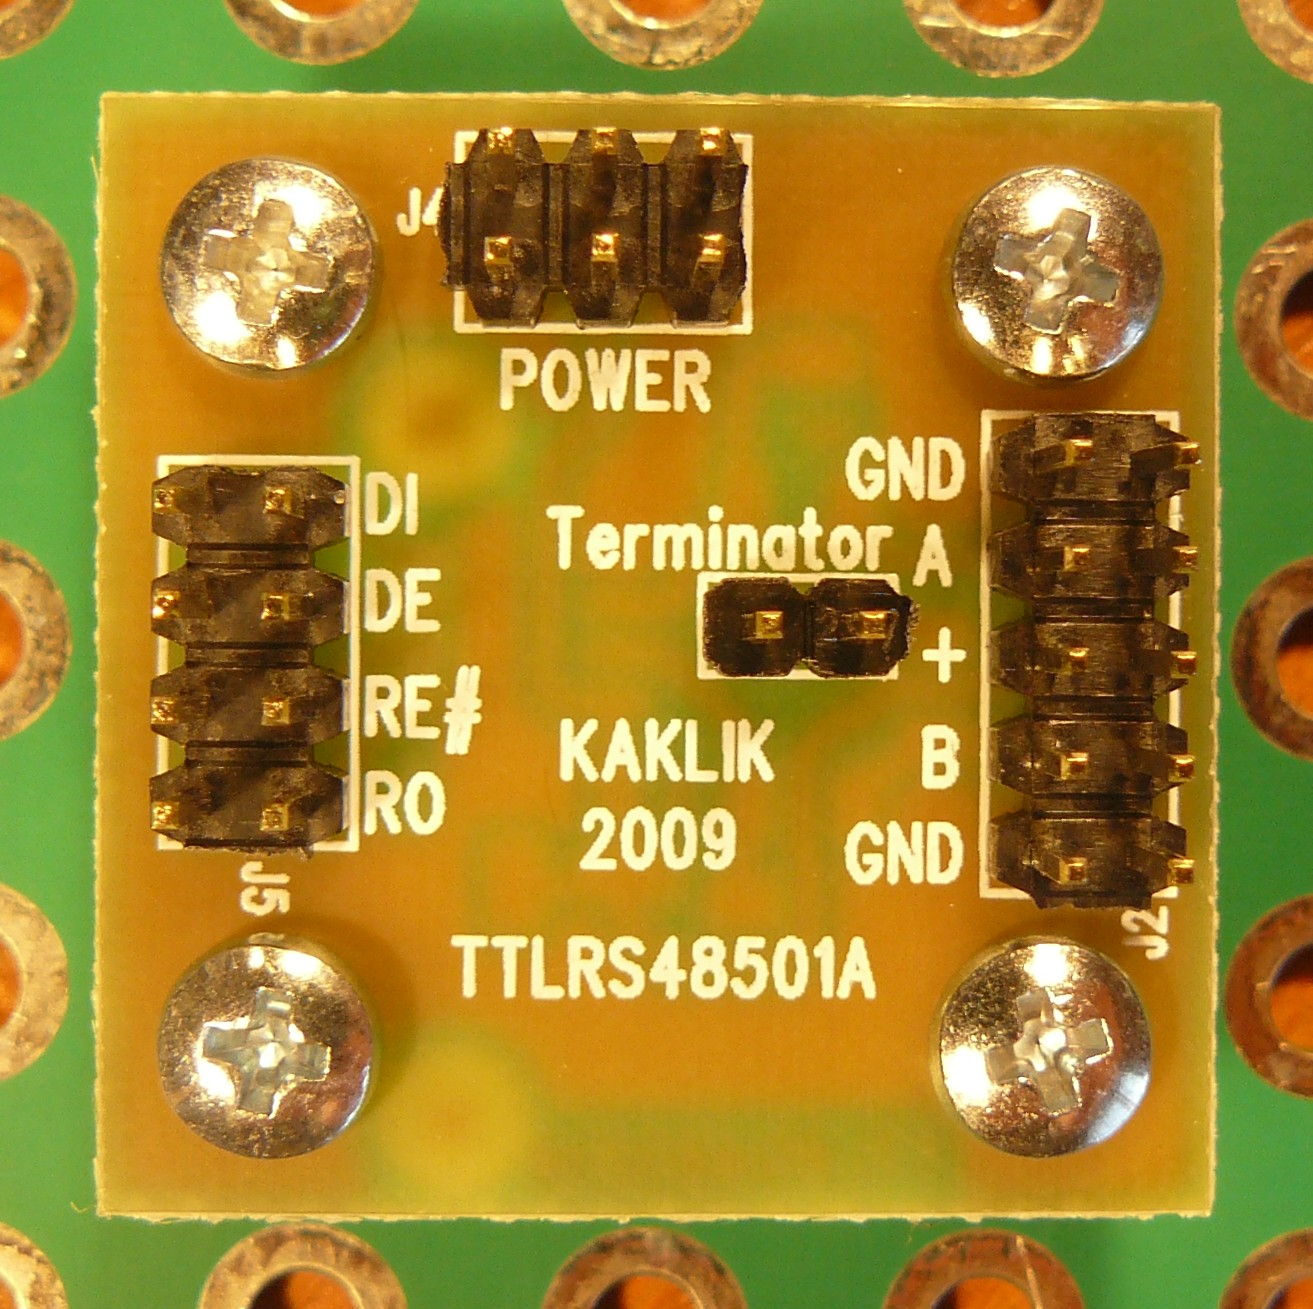
\includegraphics [width=80mm] {TTLRS48501A_Top_Big.JPG} 
\end{center}
\end{figure}

\tableofcontents


\section{Technické parametry}
\begin{table}[htbp]
\begin{center}
\begin{tabular}{|c|c|c|}
\hline
\multicolumn{1}{|c|}{Parametr} & \multicolumn{1}{|c|}{Hodnota} & \multicolumn{1}{|c|}{Poznámka} \\ \hline
Napájecí napětí & +5V &  30 mA \\ \hline
Pracovní napětí  vstupů & do +10V &  \\ \hline
Maximální budící proud  & 60 mA & \\ \hline
\end{tabular}
\end{center}
\end{table}

\newpage
\section{Popis konstrukce}

\subsection{Zapojení}

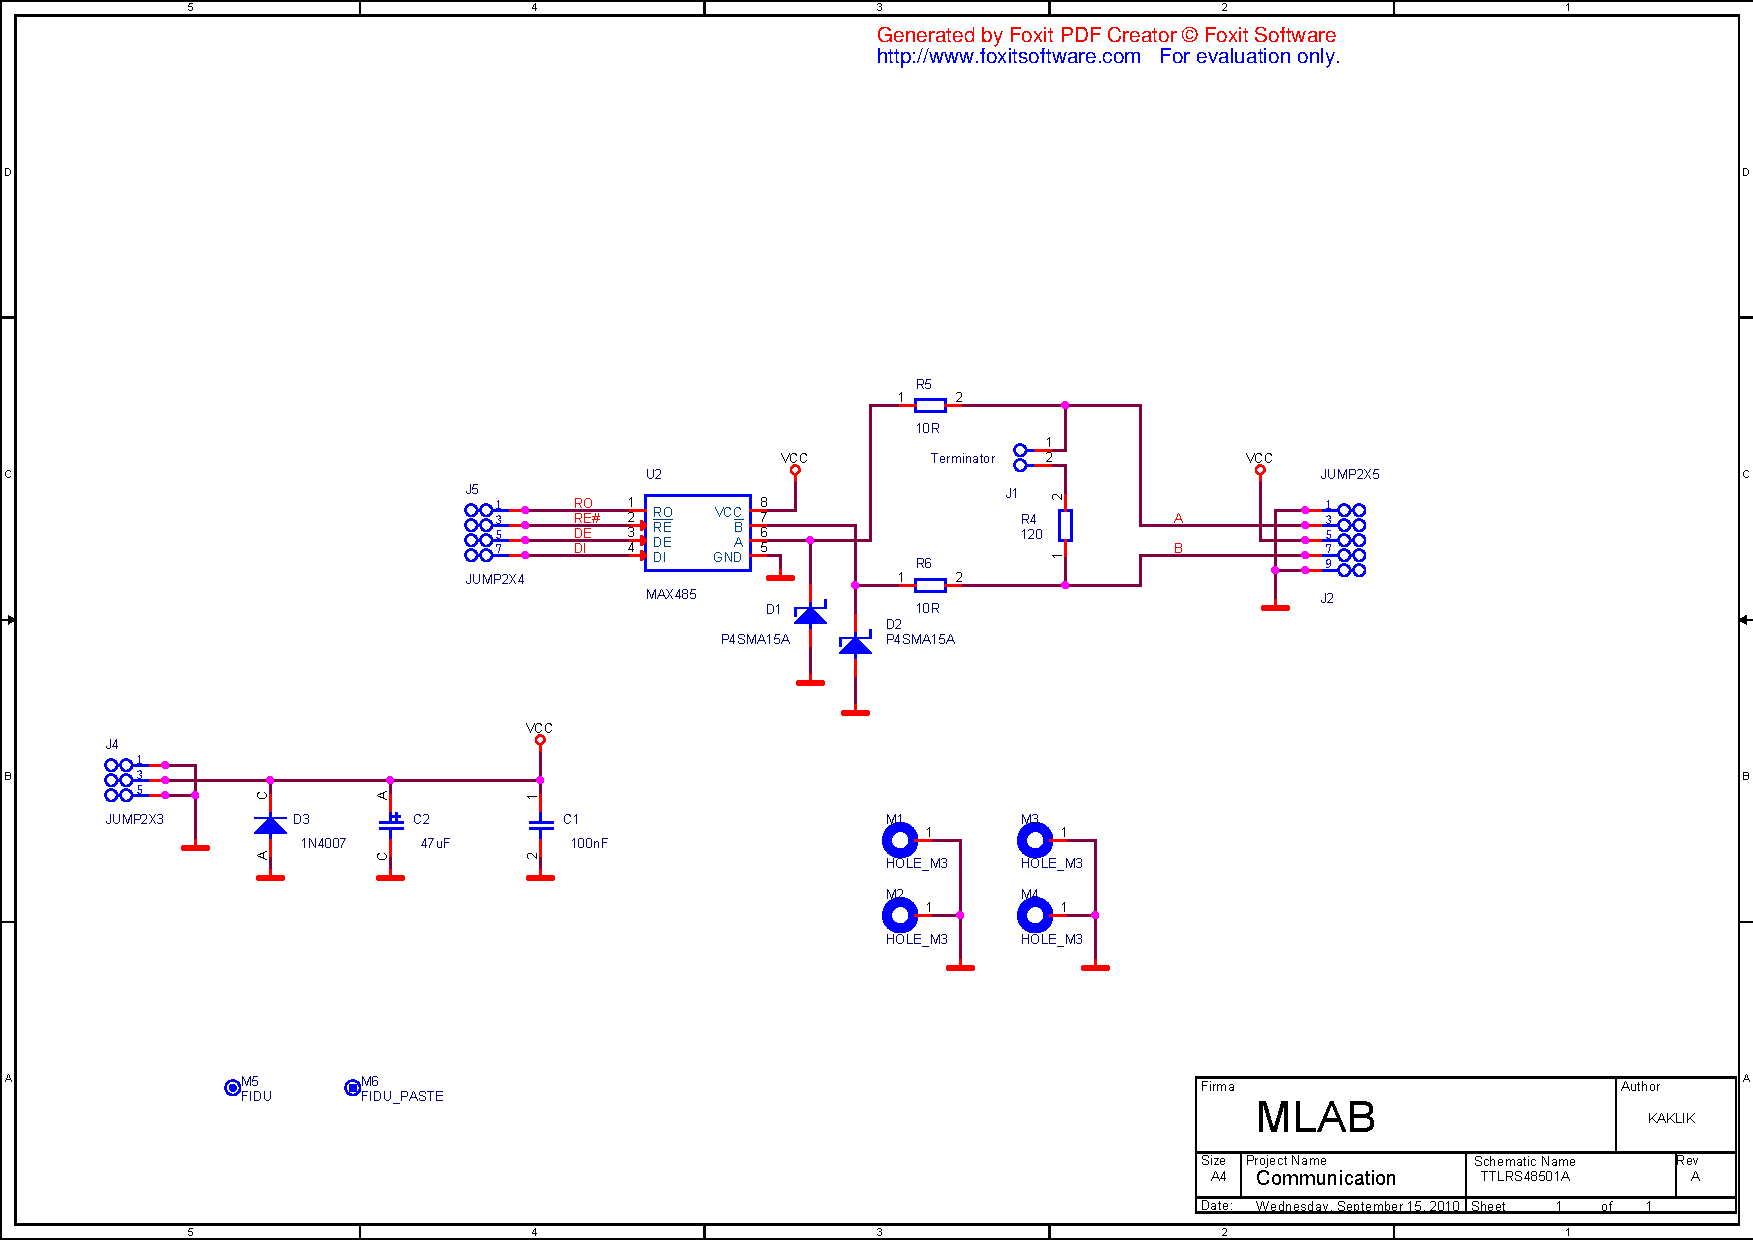
\includepdf[pages={1},landscape=true]{../../SCH/TTLRS48501A.pdf}

\subsection{Odrušení}

\subsection{Mechanická konstrukce}

\section{Výroba a testování}

\subsubsection{Osazení}

\subsubsection{Nastavení}

\section{Programové vybavení}


\begin{thebibliography}{99}
%\bibitem{DR2G}{Původní konstrukce} 
%\href{http:// odkaz na nejakou zajimavou konstrukci}{odkaz na nejakou zajimavou konstrukci}

\end{thebibliography}
\end{document}